\documentclass[tikz]{standalone}
\input{preamble.tex}

% TikZ libraries
\usetikzlibrary{shapes, fadings, backgrounds, calc, decorations.markings, arrows.meta}

% Style definitions based on reference
\tikzset{
    super thick/.style={line width=3pt},
    shaded/.style={fill=gray!25},
    interior/.style={fill=pink!40},
    edge/.style={red},
    interior_cut/.style={fill=blue!30},
    edge_cut/.style={blue},
    seam/.style={thick, blue!80!black},
    arrow_label/.style={midway, above, font=\small\bfseries, align=center},
    main_label/.style={font=\large\bfseries}
}

\begin{document}

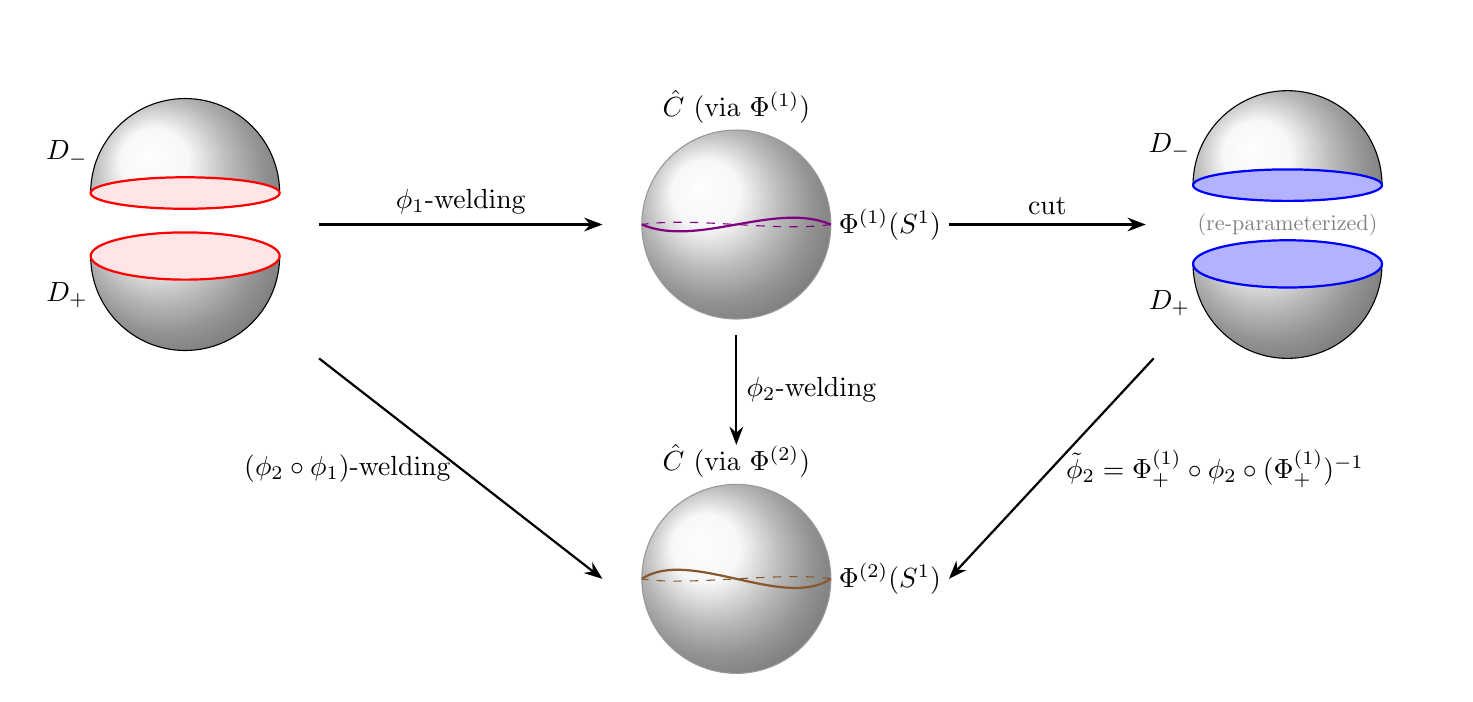
\begin{tikzpicture}[>=Stealth]

    % --- DEFINITIONS FOR REUSABLE SHAPES ---

    % 1. Top Hemisphere (D_+) - Seeing the bottom opening
    \def\drawDplus#1#2#3{
        \begin{scope}[shift={#1}]
            % Shell
            \begin{scope}
                \clip (-2,0) rectangle (2,2);
                \shade[ball color=gray!10, opacity=0.8] (0,0) circle (1.2);
            \end{scope}
            % \fill[gray!25] (1.2,0) arc(0:180:1.2) -- cycle;
            \draw (1.2,0) arc(0:180:1.2);
            % Opening (Bottom face)
            \fill[#2] (0,0) ellipse (1.2 and 0.2);
            \draw[thick, #3] (0,0) ellipse (1.2 and 0.2);
            % Label
            \node at (-1.5, 0.5) {$D_-$};
        \end{scope}
    }

    % 2. Bottom Hemisphere (D_-) - Seeing the top opening
    \def\drawDminus#1#2#3{
        \begin{scope}[shift={#1}]
            % Shell
            \begin{scope}
                \clip (-2,-2) rectangle (2,0);
                \shade[ball color=gray!10, opacity=0.8] (0,0) circle (1.2);
            \end{scope}
            % \fill[gray!25] (1.2,0) arc(0:-180:1.2) -- cycle;
            \draw (1.2,0) arc(0:-180:1.2);
            % Opening (Top face)
            \fill[#2] (0,0) ellipse (1.2 and 0.3);
            \draw[thick, #3] (0,0) ellipse (1.2 and 0.3);
            % Label
            \node at (-1.5, -0.5) {$D_+$};
        \end{scope}
    }

    % 3. Welded Sphere (Generic)
    \def\drawSphere#1#2{ % #1=position, #2=seam variation
        \begin{scope}[shift={#1}]
            % Sphere body
            \shade[ball color=gray!10, opacity=0.8] (0,0) circle (1.2);
            \draw[gray!80] (0,0) circle (1.2);
            
            % Seam (The welding curve)
            \ifnum#2=1
                % Simple seam (f-welding)
                \draw[thick, violet] (-1.2,0) .. controls (-0.5,-0.3) and (0.5,0.3) .. (1.2,0);
                \draw[dashed, violet, thin] (1.2,0) .. controls (0.5,-0.1) and (-0.5,0.1) .. (-1.2,0);
                \node at (0, 1.5) {$\hat{\mathbb{C}}$ (via $\Phi^{(1)}$)};
            \else
                % Complex seam (g o f welding)
                \draw[thick, brown!70!black] (-1.2,0) .. controls (-0.6,0.4) and (0.6,-0.4) .. (1.2,0);
                \draw[dashed, brown!70!black, thin] (1.2,0) .. controls (0.6,0.1) and (-0.6,-0.1) .. (-1.2,0);
                \node at (0, 1.5) {$\hat{\mathbb{C}}$ (via $\Phi^{(2)}$)};
            \fi
        \end{scope}
    }

    % --- DRAWING THE DIAGRAM ---

    % Coordinates
    \coordinate (TL) at (0, 4.5);   % Top Left Center
    \coordinate (TM) at (7, 4.5);   % Top Right Center
    \coordinate (TR) at (14, 4.5);   % Top Right Center
    \coordinate (BL) at (0, 0);   % Bottom Left Center
    \coordinate (BM) at (7, 0);   % Bottom Right Center
 

    % --- TOP ROW (f-welding) ---
    
    % Top Left: Disjoint Disks
    \drawDplus{($(TL)+(0, 0.4)$)}{interior}{edge}
    \drawDminus{($(TL)+(0, -0.4)$)}{interior}{edge}
    
    % Arrow Top
    \draw[->, thick] ($(TL)+(1.7,0)$) -- ($(TM)+(-1.7,0)$) node[midway, above] {$\phi_1$-welding};

    % Top Middle: Sphere 1
    \drawSphere{(TM)}{1}
    \node at ($(TM)+(1.95,0)$) {$\Phi^{(1)}(S^1)$};

    % Top Right: Sphere 1
    \drawDplus{($(TR)+(0, 0.5)$)}{interior_cut}{edge_cut}
    \drawDminus{($(TR)+(0, -0.5)$)}{interior_cut}{edge_cut}
    \node[gray, scale=0.8] at ($(TM)+(7,0)$) {(re-parameterized)};

    \draw[->, thick] ($(TM)+(2.7,0)$) -- ($(TR)-(1.8, 0)$) node[midway, above] {cut};


    % --- BOTTOM ROW ---

    % Bottom Right: Sphere 2
    \drawSphere{(BM)}{2}
    \node at ($(BM)+(1.95,0)$) {$\Phi^{(2)}(S^1)$};


    % --- VERTICAL TRANSITIONS ---

    % Right Vertical Arrow (The map between spheres, g)
    \draw[->, thick] ($(TM)-(0, 1.4)$) -- ($(BM)+(0, 1.7)$) node[midway, right] {$\phi_2$-welding};
    
    % Left Vertical Arrow (The map between disks, g_bar)
    \draw[->, thick] ($(TL)+(1.7,-1.7)$) -- ($(BM)+(-1.7,0)$) node[midway, left] {$(\phi_2 \circ \phi_1)$-welding};

    \draw[->, thick] ($(TR)-(1.7,1.7)$) -- ($(BM)+(2.7,0)$) node[midway, right] {$\,\tilde{\phi}_2 = \Phi_+^{(1)} \circ \phi_2 \circ (\Phi_+^{(1)})^{-1}$};

\end{tikzpicture}
\end{document}